% this file is encoded in utf-8
% v1.7

\documentclass[12pt, a4paper]{ntust_report} 

\usepackage{fontspec}   %加這個就可以設定字體 
\usepackage{xeCJK}       %讓中英文字體分開設置 
\setmainfont{Arial}            %設定主要字型,也就是英文字型 
%\setCJKmainfont{DFKai-SB}     %設定中文字型 (windows:預設為標楷體)
\setCJKmainfont{LiHei Pro}     %設定中文字型 (OS X:預設為儷黑)
 
\XeTeXlinebreaklocale "zh"                %這兩行一定要加,中文才能自動換行 
\XeTeXlinebreakskip = 0pt plus 1pt       %這兩行一定要加,中文才能自動換行




% 除非校方修改了論文格式 (margins, header, footer, 浮水印)
% 或者需要增加所用的 LaTeX 套件,
% 或者要改預設中文字型、編碼
% 否則毋須修改本檔內容
% 論文撰寫,請修改以 my_  開頭檔名的各檔案

\usepackage{CJK}  %%% ZZZ %%% macro for Chinese/Japanese/Korean processing
\usepackage[nospace]{cite}  % for smart citation
\usepackage{geometry}  % for easy margin settings
\usepackage{subfigure}  % for subfigure
%
% margins setting
\geometry{verbose,a4paper,tmargin=3.5cm,bmargin=2cm,lmargin=3cm,rmargin=3cm}
%
\usepackage{amsmath} % 各式 AMS 數學功能
\usepackage{amssymb} % 各式 AMS 數學符號
\usepackage{mathrsfs} %草寫體數學符號,在數學模式裡用 \mathscr{E} 得草寫 E
\usepackage{listings} % 程式列表套件
%
% listing setting
\lstset{breaklines=true,% 過長的程式行可斷行
extendedchars=false,% 中文處理不需要 extendedchars
texcl=true,% 中文註解需要有 TeX 處理過的 comment line, 所以設成 true
comment=[l]\%\%,% 以雙「百分號」做為程式中文註解的起頭標記,配合 MATLAB
basicstyle=\small,% 小號字體, 約 10 pt 大小
commentstyle=\upshape,% 預設是斜體字,會影響註解裏的英文,改用正體
%language=Octave % 會將一些 octave 指令以粗體顯示
}

\usepackage{url} % 在文稿中引用網址,可以用 \url{http://www.ntust.edu.tw} 方式

% 插圖套件 graphicx
% 使用者工作流程是用 pdftex 還是 latex + dvipdfmx?
% 視情況而有不同的參數
% 這裡作自動判斷
% 參考自
% http://www.tex.ac.uk/cgi-bin/texfaq2html?label=ifpdf

\ifx\pdfoutput\undefined
  % not running pdftex
  \usepackage[dvipdfm]{graphicx}
\else
  \ifx\pdfoutput\relax
    % not running pdftex
    \usepackage[dvipdfm]{graphicx}
  \else
    % running pdftex, with...
    \ifnum\pdfoutput>0
      % ... PDF output
      \usepackage[pdftex]{graphicx}
    \else
      %...DVI output
      \usepackage[dvipdfm]{graphicx}
    \fi
  \fi
\fi

\usepackage{fancyhdr}  % 借用增強功能型 header 套件來擺放浮水印 
% (佔用了 central header)
% 不需要浮水印的使用者仍可利用此套件,產生所需的 header, footer
%
% 啟動 fancy header/footer 套件
\pagestyle{fancy}
\fancyhead{}  % reset left, central, right header to empty
\fancyfoot[C]{\thepage} %中間 footer 擺放頁碼
\renewcommand{\headrulewidth}{0pt} % header 的直線; 0pt 則無線

% 如果不需要任何浮水印,則請把下列介於 >>> 與 <<< 之間
% 的文字行關掉 (行首加上百分號)
%% 浮水印 >>> 
%
% this file is encoded in utf-8
% v1.7
% 如果浮水印不是全篇需要,請把下列介於 >>> 與 <<<
% 的「全篇浮水印專用碼」關掉 (行首加百分號)
% 參考自 Keith Reckdahl 寫的 "Using Imported Graphics in LATEX2e" (epslatex.pdf) p.39
% 如果只有特定頁需要浮水印
% 則依該頁屬性使用下列之一的命令 
% 普通頁命令 \thispagestyle{WaterMarkPage}
% plain 頁命令 \thispagestyle{PlainWaterMarkPage}
% empty 頁命令 \thispagestyle{EmptyWaterMarkPage}


% 將重複使用的浮水印章
% 圖檔是 my_watermark.xxx
% 副檔名可以不加,可以是 latex 系統能處裡的任何格式:pdf, gif, png, jpg, eps, ...
% 某些圖檔格式在某些工作流程可能需要作前置處裡。
% 例如,pdflatex 無法直接處理 eps 檔
%  latex + dvipdfmx 無法直接處理 pdf, gif, png, jpg, 需要用 ebb 小工具程式
%  對圖檔產生 .bb 對應檔。
% old code
%\newsavebox{\mywatermark}
%\sbox{\mywatermark}{\includegraphics[keepaspectratio,%
%height=0.8\textheight,%
%width=0.8\textwidth]{my_watermark}}
% new code
\newsavebox{\mywatermark}
\sbox{\mywatermark}{
\includegraphics[keepaspectratio,
width=2.5cm]{watermark/ntust_watermark.eps}}


% 將 central header 擺放浮水印的巨集指令
\newcommand{\PlaceWaterMark}{\fancyhead[C]{\setlength{\unitlength}{1in}%
\begin{picture}(0,0)%
%\put(-2.2,-6){\usebox{\mywatermark}}% old code
\put(-0.5,-6.2){\usebox{\mywatermark}}% new code
\end{picture}}%
}

\fancyhead{}  % reset left, central, right header to empty
%% 如果不需整篇論文都要浮水印
%% 則下面  >>> 與 <<< 之間的程式碼請關閉
%% >>> 全篇浮水印
\PlaceWaterMark  % 每一頁都有浮水印 (除了 plain、empty 頁以外)

% 重新定義 plain 頁面
% 每張 plain 頁面 (每一章的第一頁) 也加浮水印

\fancypagestyle{plain}{%
\fancyhead{}%
\PlaceWaterMark%
\fancyfoot{}%
\fancyfoot[C]{\thepage}
\renewcommand{\headrulewidth}{0pt}%
\renewcommand{\footrulewidth}{0pt}%
}
%% <<< 全篇浮水印

%% 如果只有一、兩頁需要有浮水印
%% 可以在該頁 (有頁碼) 使用 \thispagestyle{WaterMarkPage}
%% 此命令不影響原有的 header、footer
\fancypagestyle{WaterMarkPage}{%
\PlaceWaterMark%
}

%% 如果只有一、兩頁 plain 頁需要有浮水印 (如 摘要、自傳等)
%% 可以在該頁 (有頁碼) 使用 \thispagestyle{PlainWaterMarkPage}
%% 只有頁碼與浮水印,沒有其他的 header、footer
%% 等同於 plain page style + water mark
\fancypagestyle{PlainWaterMarkPage}{%
\fancyhead{}%
\PlaceWaterMark%
\fancyfoot{}%
\fancyfoot[C]{\thepage}
\renewcommand{\headrulewidth}{0pt}%
\renewcommand{\footrulewidth}{0pt}%
}

%% 如果只有一、兩頁 empty 頁需要有浮水印 (如封面、書名頁)
%% 可以在該頁 (無頁碼) 使用 \thispagestyle{EmptyWaterMarkPage}
%% 等同於 empty page style + water mark
\fancypagestyle{EmptyWaterMarkPage}{%
\fancyhead{}%
\PlaceWaterMark%
\fancyfoot{}%
\renewcommand{\headrulewidth}{0pt}%
\renewcommand{\footrulewidth}{0pt}%
}

%% <<< 浮水印



% global page layout
\newcommand{\mybaselinestretch}{1.5}  %行距 1.5 倍 + 20%, (約為 double space)
\renewcommand{\baselinestretch}{\mybaselinestretch}  % 論文行距預設值
\parskip=2ex  % 段落之間的間隔為兩個 x 的高度
\parindent = 0Pt  % 段首內縮由 CJK 控制,所以這裡就設成不內縮

%%%%%%%%%%%%%%%%%%%%%%%%%%%%%
%  end of preamble
%%%%%%%%%%%%%%%%%%%%%%%%%%%%%  %基本的環境設定  無需改變  

\begin{document}



	% 下列中文名詞的定義,如果以註解方式關閉取消,
% 則會以系統原先的預設值 (英文) 替代
% 名詞 \prechaptername 預設值為 Chapter
% 名詞 \postchaptername 預設值為空字串
% 名詞 \tablename 預設值為 Table
% 名詞 \figurename 預設值為 Figure
\renewcommand\prechaptername{Chapter} % 出現在每一章的開頭的「第 x 章」
\renewcommand\postchaptername{}
\renewcommand{\tablename}{Table} % 在文章中 table caption 會以「表 x」表示
\renewcommand{\figurename}{Figure} % 在文章中 figure caption 會以「圖 x」表示

% 下列中文名詞的定義,用於論文固定的各部分之命名 (出現於目錄與該頁標題)
\newcommand{\nameInnerCover}{教授推薦書}
\newcommand{\nameCommitteeForm}{論文口試委員審定書}
\newcommand{\nameCopyrightForm}{授權書}
\newcommand{\nameCabstract}{中文摘要}
\newcommand{\nameEabstract}{Abstract}
\newcommand{\nameAckn}{Acknowledgment}
\newcommand{\nameToc}{Table of contents}
\newcommand{\nameLot}{List of Tables}
\newcommand{\nameTof}{List of Figures}
%\newcommand{\nameSlist}{符號說明}
\newcommand{\nameRef}{References}
%\newcommand{\nameVita}{自傳}
 %在此檔案處定義文章中的中文名詞

	%----------------------------------------------------------------------------------------------------------------------------------------------------------
	%%% 以下是載入前頁、本文、後頁
	% 此行請勿更動

	%----------------------------------------------------------------------------------------------------------------------------------------------------------
	% front matter 前頁
	% 包括封面、書名頁、中文摘要、英文摘要、誌謝、目錄、表目錄、圖目錄、符號說明
	% 在撰寫各章草稿時,可以把此部份「關掉」,以節省無謂的編譯時間。
	% 實際內容由
	%    my_names.tex, my_cabstract.tex, my_eabstract.tex, my_ackn.tex, my_symbols.tex
	% 決定
	% ntust_frontpages.tex 此檔只提供整體架構的定義,不需更動
	% 在撰寫各章草稿時,可以把此部份「關掉」,以節省無謂的編譯時間。
	
	%
% this file is encoded in utf-8
% v1.7
% do not change the content of this file
% unless the thesis layout rule is changed
% 無須修改本檔內容,除非校方修改了
% 封面、書名頁、中文摘要、英文摘要、誌謝、目錄、表目錄、圖目錄、符號說明
% 等頁之格式
% this file is encoded in utf-8
%v1.7

% make the line spacing in effect
\renewcommand{\baselinestretch}{\mybaselinestretch}
\large % it needs a font size changing command to be effective

% default variables definitions
% 注意!!此處只是預設值,不需更改此處
% 請更改 my_names.tex 內容
\newcommand\cTitle{論文題目}
\newcommand\eTitle{MY THESIS TITLE}
\newcommand\myCname{王鐵雄}
\newcommand\myEname{Aron Wang}
\newcommand\myStudentID{M9315048}
\newcommand\advisorCnameA{南宮明博士}
\newcommand\advisorEnameA{Dr.~Ming Nangong}
\newcommand\advisorCnameB{李斯坦博士}
\newcommand\advisorEnameB{Dr.~Stein Lee}
\newcommand\advisorCnameC{徐 石博士}
\newcommand\advisorEnameC{Dr.~Sean~Hsu}
\newcommand\univCname{國立台灣科技大學}
\newcommand\univEname{National Taiwan University of science and technology}
\newcommand\deptCname{光電工程研究所}
\newcommand\fulldeptEname{Graduate School of Electro-Optical Engineering}
\newcommand\deptEname{Electro-optical Engineering}
\newcommand\collEname{College of Engineering}
\newcommand\degreeCname{碩士}
\newcommand\degreeEname{Master of Science}
\newcommand\cYear{九十四}
\newcommand\cMonth{六}
\newcommand\cDay{十}
%\newcounter{eYear}
\newcommand\eYear{2006}
\newcommand\eMonth{June}
\newcommand\ePlace{Chungli, Taoyuan, Taiwan}


 % user's names; to replace those default variable definitions
%
% this file is encoded in utf-8
% v1.7
% 填入你的論文題目、姓名等資料
% 如果題目內有必須以數學模式表示的符號,請用 \mbox{} 包住數學模式,如下範例
% 如果中文名字是單名,與姓氏之間建議以全形空白填入,如下範例
% 英文名字中的稱謂,如 Prof. 以及 Dr.,其句點之後請以不斷行空白~代替一般空白,如下範例
% 如果你的指導教授沒有如預設的三位這麼多,則請把相對應的多餘教授的中文、英文名
%    的定義以空的大括號表示
%    如,\renewcommand\advisorCnameB{}
%          \renewcommand\advisorEnameB{}
%          \renewcommand\advisorCnameC{}
%          \renewcommand\advisorEnameC{}

% 論文題目 (中文)
\renewcommand\cTitle{%我的碩士論文題目 
可驗證之安全系統的應用
}

% 論文題目 (英文)
\renewcommand\eTitle{%My Thesis Title  
A Verifiable Secure protocol in a Secure System 
%My Thesis Title  \mbox{$\cal{H}_\infty$} and \mbox{Al$_x$Ga$_{1-x}$As}
}

% 我的姓名 (中文)
\renewcommand\myCname{王大明}

% 我的姓名 (英文)
\renewcommand\myEname{Da-Ming Wang}

%我的學號
\renewcommand\myStudentID{M1915001}

% 指導教授A的姓名 (中文)
\renewcommand\advisorCnameA{陳明明 博士}

% 指導教授A的姓名 (英文)
\renewcommand\advisorEnameA{Dr.~Ming-Ming Cheng}

% 指導教授B的姓名 (中文)
\renewcommand\advisorCnameB{}

% 指導教授B的姓名 (英文)
\renewcommand\advisorEnameB{}

% 指導教授C的姓名 (中文)
\renewcommand\advisorCnameC{}

% 指導教授C的姓名 (英文)
\renewcommand\advisorEnameC{}

% 校名 (中文)
\renewcommand\univCname{國立台灣科技大學}

% 校名 (英文)
%\renewcommand\univEname{National Taiwan University of science and technology}

% 系所名 (中文)
\renewcommand\deptCname{資~訊~工~程~系}

% 系所全名 (英文)
%\renewcommand\fulldeptEname{Graduate School of Electro-Optical Engineering}

% 系所短名 (英文, 用於書名頁學位名領域)
%\renewcommand\deptEname{Electro-Optical Engineering}

% 學院英文名 (如無,則以空的大括號表示)
%\renewcommand\collEname{College of Electrical and Communication Engineering}

% 學位名 (中文)
\renewcommand\degreeCname{碩士}

% 學位名 (英文)
%\renewcommand\degreeEname{Master of Science}

% 口試年份 (中文、民國)
\renewcommand\cYear{九十八}

% 口試月份 (中文)
\renewcommand\cMonth{七} 

% 口試月份 (中文)
\renewcommand\cDay{七} 

% 口試年份 (阿拉伯數字、西元)
%\renewcommand\eYear{2009} 

% 口試月份 (英文)
%\renewcommand\eMonth{July}

% 學校所在地 (英文)
%\renewcommand\ePlace{Taipei, Taiwan}

%畢業級別;用於書背列印;若無此需要可忽略
\newcommand\GraduationClass{95}

%%%%%%%%%%%%%%%%%%%%%%
\newcommand\itsempty{}
%%%%%%%%%%%%%%%%%%%%%%%%%%%%%%%
%       ntust cover 封面
%%%%%%%%%%%%%%%%%%%%%%%%%%%%%%%
%
\begin{titlepage}
% no page number
% next page will be page 1

% aligned to the center of the page
\begin{center}
% font size (relative to 12 pt):
% \large (14pt) < \Large (18pt) < \LARGE (20pt) < \huge (24pt)< \Huge (24 pt)
%



\begin{figure}[htbp]
	\begin{minipage}[b]{5cm} 
		\raggedright
		
\includegraphics[width=1.5in]{frontpages/ntust_logo.eps}
		\label{fig:ntust_logo}
	\end{minipage}% 
	\begin{minipage}[b]{0.5\textwidth} 
	\centering
	\makebox[3cm][c]{\Huge{\univCname}}\\  %顯示中文校名
	\vspace{0.5cm}
	\makebox[3cm][c]{\Huge{\deptCname}}\\ %顯示中文系所名
	\vspace{0.5cm}
	\end{minipage}%
\\ 
\rule{16cm}{3pt}
\end{figure}
%\hfill


\vspace{1cm}
\makebox[6cm][s]{\textbf{\Huge{\degreeCname 論文}}}\\ %顯示論文種類 (中文)
\vspace{1cm}
%
% Set the line spacing to single for the titles (to compress the lines)
\renewcommand{\baselinestretch}{1}   %行距 1 倍
%\large % it needs a font size changing command to be effective
\Large{\cTitle}\\  % 中文題目
%
\vspace{1cm}
%
\Large{\eTitle}\\ %英文題目
\vspace{5cm}
% \makebox is a text box with specified width;
% option s: stretch
% use \makebox to make sure
% 「研究生:」 與「指導教授:」occupy the same width
\hspace{4.5cm} \makebox[3cm][s]{\Large{研 究 生:}}
\Large{\myCname}  % 顯示作者中文名
\hfill \makebox[1cm][s]{}\\
%
\vspace{0.3cm}
\hspace{4.5cm} \makebox[3cm][s]{\Large{學號:}}
\Large{\myStudentID}  %顯示指導教授A中文名
\hfill \makebox[1cm][s]{}\\
%
\vspace{1cm}
\hspace{4.5cm} \makebox[3cm][s]{\Large{指導教授:}}
\Large{\advisorCnameA}  %顯示指導教授A中文名
\hfill \makebox[1cm][s]{}\\
%
% 判斷是否有共同指導的教授 B
\ifx \advisorCnameB  \itsempty
\relax % 沒有 B 教授,所以不佔版面,不印任何空白
\else
% 共同指導的教授 B
\hspace{4.5cm} \makebox[3cm][s]{}
\Large{\advisorCnameB}  %顯示指導教授B中文名
\hfill \makebox[1cm][s]{}\\
\fi
%
% 判斷是否有共同指導的教授 C
\ifx \advisorCnameC  \itsempty
\relax % 沒有 C 教授,所以不佔版面,不印任何空白
\else
% 共同指導的教授 C
\hspace{4.5cm} \makebox[3cm][s]{}
\Large{\advisorCnameC}  %顯示指導教授C中文名
\hfill \makebox[1cm][s]{}\\
\fi
%
\vfill
\makebox[10cm][s]{\Large{中華民國\cYear 年\cMonth 月\cDay 日}}%
%
\end{center}
% Resume the line spacing to the desired setting
\renewcommand{\baselinestretch}{\mybaselinestretch}   %恢復原設定
% it needs a font size changing command to be effective
% restore the font size to normal
\normalsize
\end{titlepage}
%%%%%%%%%%%%%%

%% 從摘要到本文之前的部份以小寫羅馬數字印頁碼
% 但是從「書名頁」(但不印頁碼) 就開始計算
\setcounter{page}{1}
%\pagenumbering{roman}
\pagenumbering{arabic}
%%%%%%%%%%%%%%%%%%%%%%%%%%%%%%%
%       指導教授推薦書 
%%%%%%%%%%%%%%%%%%%%%%%%%%%%%%%
%
% insert the printed standard form when the thesis is ready to bind
% 在口試完成後,再將已簽名的推薦書放入以便裝訂
% create an entry in table of contents for 推薦書
% 目前送出空白頁
\newpage{\thispagestyle{empty}\addcontentsline{toc}{chapter}{\nameInnerCover}\mbox{}\clearpage}
%\newpage

% 判斷是否要浮水印?
\ifx\mywatermark\undefined 
  \thispagestyle{empty}  % 無頁碼、無 header (無浮水印)
\else
  \thispagestyle{EmptyWaterMarkPage} % 無頁碼、有浮水印
\fi

%%%%%%%%%%%%%%%%%%%%%%%%%%%%%%%%%%%%%%%%%%%%%%%%%%%%%%%%%%%%%%%
%%no page number
%% create an entry in table of contents for 書名頁
%\addcontentsline{toc}{chapter}{\nameInnerCover}
%
%
%% aligned to the center of the page
%\begin{center}
%% font size (relative to 12 pt):
%% \large (14pt) < \Large (18pt) < \LARGE (20pt) < \huge (24pt)< \Huge (24 pt)
%% Set the line spacing to single for the titles (to compress the lines)
%\renewcommand{\baselinestretch}{1}   %行距 1 倍
%% it needs a font size changing command to be effective
%%中文題目
%\Large{\cTitle}\\ %%%%%
%\vspace{1cm}
%% 英文題目
%\Large{\eTitle}\\ %%%%%
%%\vspace{1cm}
%\vfill
%% \makebox is a text box with specified width;
%% option s: stretch
%% use \makebox to make sure
%% 「研究生:」 與「指導教授:」occupy the same width
%\makebox[3cm][s]{\large{研 究 生:}}
%\makebox[3cm][l]{\large{\myCname}} %%%%%
%\hfill
%\makebox[2cm][s]{\large{Student: }}
%\makebox[5cm][l]{\large{\myEname}}\\ %%%%%
%%
%%\vspace{1cm}
%%
%\makebox[3cm][s]{\large{指導教授:}}
%\makebox[3cm][l]{\large{\advisorCnameA}} %%%%%
%\hfill
%\makebox[2cm][s]{\large{Advisor: }}
%\makebox[5cm][l]{\large{\advisorEnameA}}\\ %%%%%
%%
%% 判斷是否有共同指導的教授 B
%\ifx \advisorCnameB  \itsempty
%\relax % 沒有 B 教授,所以不佔版面,不印任何空白
%\else
%%共同指導的教授B
%\makebox[3cm][s]{}
%\makebox[3cm][l]{\large{\advisorCnameB}} %%%%%
%\hfill
%\makebox[2cm][s]{}
%\makebox[5cm][l]{\large{\advisorEnameB}}\\ %%%%%
%\fi
%%
%% 判斷是否有共同指導的教授 C
%\ifx \advisorCnameC  \itsempty
%\relax % 沒有 C 教授,所以不佔版面,不印任何空白
%\else
%%共同指導的教授C
%\makebox[3cm][s]{}
%\makebox[3cm][l]{\large{\advisorCnameC}} %%%%%
%\hfill
%\makebox[2cm][s]{}
%\makebox[5cm][l]{\large{\advisorEnameC}}\\ %%%%%
%\fi
%%
%% Resume the line spacing to the desired setting
%\renewcommand{\baselinestretch}{\mybaselinestretch}   %恢復原設定
%\large %it needs a font size changing command to be effective
%%
%\vfill
%\makebox[4cm][s]{\large{\univCname}}\\% 校名
%\makebox[6cm][s]{\large{\deptCname}}\\% 系所名
%\makebox[3cm][s]{\large{\degreeCname 論文}}\\% 學位名
%%
%%\vspace{1cm}
%\vfill
%\large{A Thesis}\\%
%\large{Submitted to }%
%%
%\large{\fulldeptEname}\\%系所全名 (英文)
%%
%%
%\ifx \collEname  \itsempty
%\relax % 沒有學院名 (英文),所以不佔版面,不印任何空白
%\else
%% 有學院名 (英文)
%\large{\collEname}\\% 學院名 (英文)
%\fi
%%
%\large{\univEname}\\%校名 (英文)
%%
%\large{in Partial Fulfillment of the Requirements}\\
%%
%\large{for the Degree of}\\
%%
%\large{\degreeEname}\\%學位名(英文)
%
%\large{in}\\
%%
%\large{\deptEname}\\%系所短名(英文;表明學位領域)
%%
%\large{\eMonth\ \eYear}\\%月、年 (英文)
%%
%\large{\ePlace}% 學校所在地 (英文)
%\vfill
%\large{中華民國}%
%\large{\cYear}% %%%%%
%\large{年}%
%\large{\cMonth}% %%%%%
%\large{月}\\
%\end{center}
%% restore the font size to normal
%\normalsize
%\clearpage


%%%%%%%%%%%%%%%%%%%%%%%%%%%%%%%%%%%%%%%%%%%%%%%%%%%%%%%%%%%%%%%%%%%%%
%%%%%%%%%%%%%%%%%%%%%%%%%%%%%%%
%       論文口試委員審定書 (計頁碼,但不印頁碼) 
%%%%%%%%%%%%%%%%%%%%%%%%%%%%%%%
%
% insert the printed standard form when the thesis is ready to bind
% 在口試完成後,再將已簽名的審定書放入以便裝訂
% create an entry in table of contents for 審定書
% 目前送出空白頁
\newpage{\thispagestyle{empty}\addcontentsline{toc}{chapter}{\nameCommitteeForm}\mbox{}\clearpage}


%%%%%%%%%%%%%%%%%%%%%%%%%%%%%%%
%       中文摘要 
%%%%%%%%%%%%%%%%%%%%%%%%%%%%%%%
%
\newpage
\thispagestyle{plain}  % 無 header,但在浮水印模式下會有浮水印
% create an entry in table of contents for 中文摘要
\addcontentsline{toc}{chapter}{\nameCabstract}

% aligned to the center of the page
\begin{center}
% font size (relative to 12 pt):
% \large (14pt) < \Large (18pt) < \LARGE (20pt) < \huge (24pt)< \Huge (24 pt)
% Set the line spacing to single for the names (to compress the lines)
\renewcommand{\baselinestretch}{1}   %行距 1 倍
% it needs a font size changing command to be effective
\large{\cTitle}\\  %中文題目
\vspace{0.83cm}
% \makebox is a text box with specified width;
% option s: stretch
% use \makebox to make sure
% each text field occupies the same width
\makebox[1.5cm][s]{\large{學生:}}
\makebox[3cm][l]{\large{\myCname}} %學生中文姓名
\hfill
%
\makebox[3cm][s]{\large{指導教授:}}
\makebox[3cm][l]{\large{\advisorCnameA}} \\ %教授A中文姓名
%
% 判斷是否有共同指導的教授 B
\ifx \advisorCnameB  \itsempty
\relax % 沒有 B 教授,所以不佔版面,不印任何空白
\else
%共同指導的教授B
\makebox[1.5cm][s]{}
\makebox[3cm][l]{} %%%%%
\hfill
\makebox[3cm][s]{}
\makebox[3cm][l]{\large{\advisorCnameB}}\\ %教授B中文姓名
\fi
%
% 判斷是否有共同指導的教授 C
\ifx \advisorCnameC  \itsempty
\relax % 沒有 C 教授,所以不佔版面,不印任何空白
\else
%共同指導的教授C
\makebox[1.5cm][s]{}
\makebox[3cm][l]{} %%%%%
\hfill
\makebox[3cm][s]{}
\makebox[3cm][l]{\large{\advisorCnameC}}\\ %教授C中文姓名
\fi
%
\vspace{0.42cm}
%
\large{\univCname}\large{\deptCname}\\ %校名系所名
\vspace{0.83cm}
%\vfill
\makebox[2.5cm][s]{\large{摘要}}\\
\end{center}
% Resume the line spacing to the desired setting
\renewcommand{\baselinestretch}{\mybaselinestretch}   %恢復原設定
%it needs a font size changing command to be effective
% restore the font size to normal
\normalsize
%%%%%%%%%%%%%
	
   分散式詢問及監督系統主要被用於分散式資料如檔案或是紀錄的維護上。網路內的使用者可以自系統中查詢所需資料如總和或平均值,若同時將所有原始資料做傳遞及運算,將耗費相當大的網路頻寬及運算資源。於是,內網路聚集技術被提出來降低分散式詢問及監督系統的負擔。然而,這個技術卻容易遭受安全威脅。過去的研究大多假設資料來源為可信任,並針對聚集架構進行安全性的研究。然而,我們認為聚集查詢結果應該在面對惡意攻擊者將錯誤資料置入資料串流進行聚集前,就應該具備強健的容錯能力。傳統上,一個強健的估計值被定義為即使資料來源有誤時,亦能維持一定程度正確性的聚集結果。許多常見的強健估計值是建立在有序統計學上,因此,我們將重心放在內網路計算上之有序統計的可驗證技術。此技術的挑戰為在網路遭受惡意團體介入聚集程序時,仍能確保聚集結果或近似結果的準確性。

%%%%%%%%%%%%%%%%%%%%%%%%%%%%%%%
%       英文摘要 
%%%%%%%%%%%%%%%%%%%%%%%%%%%%%%%
%
\newpage
\thispagestyle{plain}  % 無 header,但在浮水印模式下會有浮水印

% create an entry in table of contents for 英文摘要
\addcontentsline{toc}{chapter}{\nameEabstract}

% aligned to the center of the page
\begin{center}
% font size:
% \large (14pt) < \Large (18pt) < \LARGE (20pt) < \huge (24pt)< \Huge (24 pt)
% Set the line spacing to single for the names (to compress the lines)
\renewcommand{\baselinestretch}{1}   %行距 1 倍
%\large % it needs a font size changing command to be effective
\large{\eTitle}\\  %英文題目
\vspace{0.83cm}
% \makebox is a text box with specified width;
% option s: stretch
% use \makebox to make sure
% each text field occupies the same width
\makebox[2cm][s]{\large{Student: }}
\makebox[5cm][l]{\large{\myEname}} %學生英文姓名
\hfill
%
\makebox[2cm][s]{\large{Advisor: }}
\makebox[5cm][l]{\large{\advisorEnameA}} \\ %教授A英文姓名
%
% 判斷是否有共同指導的教授 B
\ifx \advisorCnameB  \itsempty
\relax % 沒有 B 教授,所以不佔版面,不印任何空白
\else
%共同指導的教授B
\makebox[2cm][s]{}
\makebox[5cm][l]{} %%%%%
\hfill
\makebox[2cm][s]{}
\makebox[5cm][l]{\large{\advisorEnameB}}\\ %教授B英文姓名
\fi
%
% 判斷是否有共同指導的教授 C
\ifx \advisorCnameC  \itsempty
\relax % 沒有 C 教授,所以不佔版面,不印任何空白
\else
%共同指導的教授C
\makebox[2cm][s]{}
\makebox[5cm][l]{} %%%%%
\hfill
\makebox[2cm][s]{}
\makebox[5cm][l]{\large{\advisorEnameC}}\\ %教授C英文姓名
\fi
%
\vspace{0.42cm}
\large{Submitted to }\large{\fulldeptEname}\\  %英文系所全名
%
\ifx \collEname  \itsempty
\relax % 如果沒有學院名 (英文),則不佔版面,不印任何空白
\else
% 有學院名 (英文)
\large{\collEname}\\% 學院名 (英文)
\fi
%
\large{\univEname}\\  %英文校名
\vspace{0.83cm}
%\vfill
%
\large{ABSTRACT}\\
%\vspace{0.5cm}
\end{center}
% Resume the line spacing the desired setting
\renewcommand{\baselinestretch}{\mybaselinestretch}   %恢復原設定
%\large %it needs a font size changing command to be effective
% restore the font size to normal
\normalsize
%%%%%%%%%%%%%

	Distributed querying and monitoring systems have been widely studied in recent years. These systems aim to maintain data sources, such as data set or log files, and allow users to query over those data sources. When the data sources are highly related and users only care some statistic results, like the sum or the average, it is consumed to transmit all data sources via the network. To minimize the network consumption, in-network aggregation technique is proposed. However, this technique is subject to some known attacks, such as the injection attack and the pollution attack. Prior works only considered the settings that data sources are trusted while the network is not. We study the way to relax the limitation and guarantee the aggregate queries robust to malicious or faulty data sources (also called polluted data sources). 

%%%%%%%%%%%%%%%%%%%%%%%%%%%%%%%
%       誌謝 
%%%%%%%%%%%%%%%%%%%%%%%%%%%%%%%
%
% Acknowledgment
\newpage
\chapter*{\protect\makebox[5cm][s]{\nameAckn}} %\makebox{} is fragile; need protect
\addcontentsline{toc}{chapter}{\nameAckn}

	首先誠摯的感謝指導教授陳明明博士,老師悉心的教導使我得以一窺WSN的深奧,不時的討論並指點我正確的方向,使我在這些年中獲益匪淺。老師對學問的嚴謹更是我輩學習的典範。
    本論文的完成另外亦得感謝老師們大力協助。因為有你們的體諒及幫忙,使得本論文能夠更完整而嚴謹。
 兩年裡的日子,實驗室裡共同的生活點滴,學術上的討論、言不及義的閒扯、讓人又愛又怕的宵夜、趕作業的革命情感、因為睡太晚而遮遮掩掩閃進實驗室........,感謝眾位學長姐、同學、學弟妹的共同砥礪,你/妳們的陪伴讓兩年的研究生活變得絢麗多彩。
	最後絕對不能忘記最了解、最支持我的家人─我的父親、母親及姊姊,在我喪失動力之時,隨時都能給予我心靈上無窮盡的關心與鼓勵,讓我有勇氣堅持到最後,完成研究的旅途。還有很多曾經幫助過我的朋友,因為有大家的幫助,我才能有今天的成果。想要感謝的人真的太多太多,就只有感謝上天了!



%%%%%%%%%%%%%%%%%%%%%%%%%%%%%%%
%       目錄 
%%%%%%%%%%%%%%%%%%%%%%%%%%%%%%%
%
% Table of contents
\newpage
\renewcommand{\contentsname}{\protect\makebox[5cm][s]{\nameToc}}
%\makebox{} is fragile; need protect
\addcontentsline{toc}{chapter}{\nameToc}
\tableofcontents

%%%%%%%%%%%%%%%%%%%%%%%%%%%%%%%
%       表目錄 
%%%%%%%%%%%%%%%%%%%%%%%%%%%%%%%
%
% List of Tables
\newpage
\renewcommand{\listtablename}{\protect\makebox[5cm][s]{\nameLot}}
%\makebox{} is fragile; need protect
\addcontentsline{toc}{chapter}{\nameLot}
\listoftables

%%%%%%%%%%%%%%%%%%%%%%%%%%%%%%%
%       圖目錄 
%%%%%%%%%%%%%%%%%%%%%%%%%%%%%%%
%
% List of Figures
\newpage
\renewcommand{\listfigurename}{\protect\makebox[5cm][s]{\nameTof}}
%\makebox{} is fragile; need protect
\addcontentsline{toc}{chapter}{\nameTof}
\listoffigures

%%%%%%%%%%%%%%%%%%%%%%%%%%%%%%%
%       演算法目錄 
%%%%%%%%%%%%%%%%%%%%%%%%%%%%%%%
%
% List of Figures
\newpage
\renewcommand{\listalgorithmname}{\protect\makebox[5cm][s]{\nameToa}}
%\makebox{} is fragile; need protect
\addcontentsline{toc}{chapter}{\nameToa}
\listofalgorithms


%%%%%%%%%%%%%%%%%%%%%%%%%%%%%%%
%       符號說明 
%%%%%%%%%%%%%%%%%%%%%%%%%%%%%%%
%
% Symbol list
% define new environment, based on standard description environment
% adapted from p.60~64, <<The LaTeX Companion>>, 1994, ISBN 0-201-54199-8
%\newcommand{\SymEntryLabel}[1]%
% {\makebox[3cm][l]{#1}}
%
%\newenvironment{SymEntry}
%   {\begin{list}{}%
%       {\renewcommand{\makelabel}{\SymEntryLabel}%
%        \setlength{\labelwidth}{3cm}%
%        \setlength{\leftmargin}{\labelwidth}%
%        }%
%   }%
%   {\end{list}}
%%
%\newpage
%\chapter*{\protect\makebox[5cm][s]{\nameSlist}} %\makebox{} is fragile; need protect
%\addcontentsline{toc}{chapter}{\nameSlist}
%%
% this file is encoded in utf-8
% v1.7
%  各符號以 \item[] 包住,然後接著寫說明
% 如果符號是數學符號,應以數學模式表示,以取得正確的字體
% 如果符號本身帶有方括號,則此符號可以用大括號 {} 包住保護
\begin{SymEntry}

\item[OLED]
Organic Light Emitting Diode

\item[$E$]
energy

\item[$e$]
the absolute value of the electron charge, $1.60\times10^{-19}\,\text{C}$
 
\item[$\mathscr{E}$]
electric field strength (V/cm)

\item[{$A[i,j]$}]
the  element of the matrix $A$ at $i$-th row, $j$-th column\\
矩陣 $A$ 的第 $i$ 列,第 $j$ 行的元素

\end{SymEntry}


\newpage
%% 論文本體頁碼回復為阿拉伯數字計頁,並從頭起算
%\pagenumbering{arabic}
%%%%%%%%%%%%%%%%%%%%%%%%%%%%%%%% 




	%----------------------------------------------------------------------------------------------------------------------------------------------------------
	% main body 論文主體。建議以「章」為檔案分割的依據。
	% 以下為建議的命名分類
	%   introduction.tex   related_work.tex  protocol.tex  evaluation.tex  conclusion.tex
	% 做為這幾個「章」的檔案名稱,並將檔案存放於資料夾 sections/ 下
	% 實際命名方式可以隨你意
	% 在撰寫各章草稿時,可以把其他章節關掉 (行首加百分號)
	%\input{example/example_body.tex}  % 所附的範例

	
\chapter{Introduction}
\label{cha:intro} 

網路發展興盛至今,小至個人,大至政府單位與各機關組織,都相當仰賴網路的使用,但許多人仍然對資安危機意識較低,針對資訊安全產品的投資也相對較少,加上對於資訊安全軟體工具缺乏有系統的整理,以致於未能有效運用。為此,本手冊蒐集整理相關開放源碼(Open Source)的資訊安全軟體工具,並透過專業人員實際操作演練,加以彙整並集結成冊,希冀透過本手冊的幫助,不僅能給予初學者對於資安工具軟體初步認識,也讓資訊從業人員在資訊安全工具上能有更多的選擇與應用。

資安開放源碼軟體的發展,往往會公開其發展技術及運用的原理,配合程式碼的開放,使得開放源碼軟體具有相當大的彈性,並根據個人使用情況所需,進行軟體的編修與整合,以求適應各種作業環境所需。使用開放源碼軟體所需負擔的金錢成本,遠低於商業付費軟體,可降低企業組織對資訊科技產品的部分支出,不需要過度仰賴軟體製造商的技術支援與更新,也能減少相對應的軟體開發時程~\cite{GarofalakisHM07}。由於目前多數的資安開放源碼軟體的開發多為國外組織,因此較缺乏中文化介面,且部分軟體工具的使用,需要具備相當程度的專業知識~\cite{MaddenFHH02},並非人人皆可輕易上手。本手冊擬透過中文化的工具介紹,減緩國內使用者入門的負擔。

由於現今網路環境日益複雜,遭受網路攻擊的事件層出不窮,網路安全越來越受到各界重視。網路掃描是網路安全的根本,也是攻擊者對目標主機進行攻擊的首要步驟,因此,了解網路掃描的攻擊與防禦,將有助於網路管理者提升網域的安全管理。此外,網路流量代表所有網路訊息的傳送,能提供管理者即時了解網路狀況,藉此檢視網路情況正常與否。本手冊將針對以上兩類的開放源碼軟體,逐一介紹其功能、安裝、操作與軟體評比,令讀者對相關的資訊軟體能有所了解,並進一步應用於資訊安全的監測與控管。以下即對網路掃描及流量監控兩大類軟體,進行整理與原理說明~\cite{KotiVDSD07, SubrPPKG06, ShengLMJ07, Wagner04}。
	
Insecure.org網站曾於2003年及2006年間調查各使用者喜愛的工具軟體,其中2006年收到3,243位受訪者的回覆,受訪對象涵括各界對資安工具有持續研究與發展的學者及廠商,包括Insecure.org自身、研究網際網路議題的機構、發展開放源碼軟體的組織,與其他著名的資安網站(如Open Source Security、Honeypots和IDS Focus等),並根據調查結果選出前100大網路安全工具(Top 100 Network Security Tools)。本手冊從中篩選了數套較廣泛應用且屬於開放源碼的工具軟體進行蒐集整理,以提供使用者參考學習使用。以下針對各工具軟體予以介紹相關的資訊安全基礎知識(包括專業術語解釋、專有名詞解析)、軟體安裝與使用方式,以及防駭相關知識。使用者將能透過本手冊掌握並熟悉更多相關熱門工具,且對資訊安全攻防技術有更進一步的認識。如表~\ref{tab:system}所示。 


\begin{table}[t!]
  \begin{center}
    \caption{The relation of aggregation overhead between different techniques}
    \label{tab:system}
    \begin{tabular}{|c|c c c|}
      \hline
       & Space usage & Communication & Query \\
       & of root aggregator & overhead & requirement \\
      \hline
      Traditional warehouse & $n$ & $O(n)$ & $O(n)$ \\
      \hline
      AM-FM sketch technique & $\log a$ & $O(\log n)$ &  $O(a\log n)$ \\
      \hline
      ``prototypical PHI query'' & $\log a$ & $O(\log n)$ & $O(\log n)$ \\
      \hline
      \end{tabular}
  \end{center}
\end{table}
	\chapter{Preliminaries}
\label{sec:preliminaries}

作業系統指紋辨識的方法,可分為主動式作業系統指紋辨識(Active OS Fingerprinting )與被動式作業系統指紋辨識(Passive OS Fingerprinting )。主動式作業系統指紋辨識,主動對目標主機送出自製的探測封包,並根據回傳的反應做判斷依據,軟體工具Nmap與Xprobe2即屬於此類。Nmap主要控制TCP的參數值,做為探測用封包;Xprobe2則是著重於送出ICMP 封包,利用邏輯樹斷定作業系統的類型。被動式作業系統指紋辨識是監聽網路上目標主機的封包往來做為判斷的依據,P0f即屬於被動式,相對於主動式作業系統指紋辨識較不易被人察覺。不論是主動式或被動式的作業系統指紋辨識,皆利用TCP/IP堆疊進行辨識,包括封包存活時間(time to live, TTL)、Window Size、最大分割大小(Maximum Segment Size)、不分段標記(Don't Fragment flag)、Window Scale Option等,因為不同的作業系統的fingerprint有所不同,所以可做為判定作業系統的依據。如圖~\ref{fig:PHI}所示。


\begin{figure}[t!]
  \begin{center}
    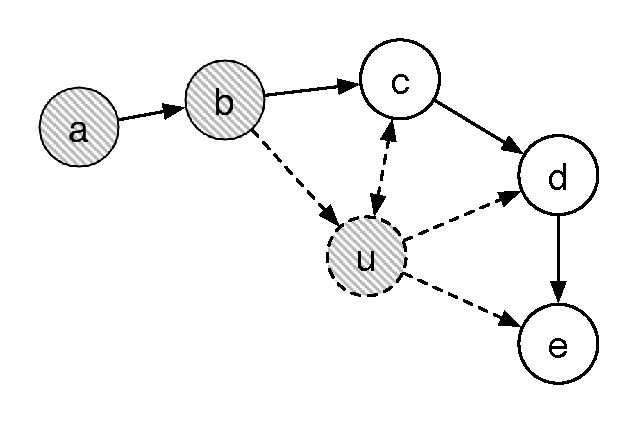
\includegraphics[width=1.0\textwidth]{figures/dyna_rm.eps}
    \caption{The diagram of ``prototypical PHI query''} 
    \label{fig:PHI}
  \end{center}
\end{figure}
	\chapter{Conclusions}
\label{cha:conclusions}


本論文蒐集了各類資訊安全工具軟體,目的是為了讓更多使用者了解資訊安全的重要性,以及如何更有效的運用網路資源。透過一系列的資訊安全基礎知識及專有名詞解釋,搭配軟體的安裝及實作步驟,讓初級使用者能更容易跨越資訊安全議題的門檻,對駭客攻防與妨駭相關知識有更深的了解。

對進階使用者而言,本手冊也針對開放源碼工具做介紹,大部分工具都有釋出其原始碼,並歡迎有能力的使用者開發出更完善的程式。另外,使用者也可以結合不同功能性的軟體,自行開發出一套符合其需求的軟體,例如利用作業系統辨識工具搭配弱點掃描工具,能夠更快的找出目標主機的系統漏洞,以發揮1+1大於2的功效。

\section{Future Work} 
%\paragraph{Future work} 
使用安全工具軟體開創一個美好和階的社會。



	%----------------------------------------------------------------------------------------------------------------------------------------------------------
	% back pages 後頁
	% 包括參考文獻、附錄、自傳
	% 實際內容由
	%    my_bib.bib, my_appendix.tex, my_vita.tex
	% 決定
	% ntust_backpages.tex 此檔只提供整體架構的定義,不需更動
	% 在撰寫各章草稿時,可以把此部份「關掉」,以節省無謂的編譯時間。
	%
% this file is encoded in utf-8
% v1.7

%%% 參考文獻
\newpage
\addcontentsline{toc}{chapter}{\nameRef}
\renewcommand{\bibname}{\protect\makebox[5cm][s]{\nameRef}}
%  \makebox{} is fragile; need protect
%\bibliographystyle{alpha}  % 使用 IEEE Trans 期刊格式
\bibliographystyle{ieeetr}  % 使用 IEEE Trans 期刊格式
\bibliography{my_bib}  %reference 所需的bib檔


%%% 附錄
%%
% this file is encoded in utf-8
% v1.7
%%% 每一個附錄 (附錄一、附錄二、...) 都要複製此段附錄編排碼做為起頭
%%% 附錄編排碼 begin >>>
\newpage
\chapter*{附錄一:MATLAB 程式列表} % 修改附錄編號與你的附錄名
\addcontentsline{toc}{chapter}{附錄一:MATLAB 程式列表} %建議此內容應與上行相同
\renewcommand{\thechapter}{一} % 如果是附錄二,則內容應為{二}

\setcounter{equation}{0} 
\setcounter{figure}{0} 
\setcounter{footnote}{0} 
\setcounter{section}{0} 
\setcounter{subsection}{0}
\setcounter{subsubsection}{0}
\setcounter{table}{0} 
%%% <<< 附錄編排碼 end

% 附錄內容開始
\lstinputlisting{example/example_prog_list.m}


%%% 如果有附錄二、三、...,則在此繼續加上「附錄編排」碼
% 每一個附錄會自動以新頁開始

%%% 自傳
%\newpage
%\chapter*{\protect\makebox[5cm][s]{\nameVita}} % \makebox{} is fragile; need protect
%\addcontentsline{toc}{chapter}{\nameVita}
%本人生於 1981 年 1 月 1 日,在桃園內壢。家裡經營電器行,上有一位姊姊。從小就喜歡拆解店裡收回的報廢家電用品,練就了一身好手藝與探究一切的好奇心。

國小就讀平鎮國小。由於把供應全校用水的抽水馬達拆開研究裝不回去,造成全校停水,廁所污穢不堪。被校長處罰掃廁所一個星期。那真是我少時年幼無知的一頁插曲。



%%%%%%%%%%%%%%%%%%%%%%%%%%%%%%%
%       授權書 (計頁碼,但不印頁碼) 
%%%%%%%%%%%%%%%%%%%%%%%%%%%%%%%
%
% insert the printed standard form when the thesis is ready to bind
% 在口試完成後,再將已簽名的授權書放入以便裝訂
% create an entry in table of contents for 授權書
% 目前送出空白頁
%\newpage{\thispagestyle{empty}\addcontentsline{toc}{chapter}{\nameCopyrightForm}\mbox{}\clearpage}





\end{document} 
 
